\section{Einleitung}
Diese Versuchsreihe befasst sich mit den verschiedenen Eigenschaften von Mikrowellenstrahlung. Mikrowellenstrahlung bezeichnet elektromagnetische Wellen im Wellenlängenbereich von etwa \SI{1}{\milli\meter} bis \SI{30}{\centi\meter}. Der Frequenzbereich von Mikrowellen beträgt etwa \SIrange{1}{300}{\giga\hertz}. Mikrowellenstrahlung findet im Alltag Einsatz in der Funkübertragung (zum Beispiel : WLAN, Mobilfunk) und im Mikrowellenherd.
\subsection{Strahldivergenz}
Der Strahlenemitter der in den Versuchen verwendet wird ist konzipiert, um einen möglichst kollimierten Strahl zu emittieren. Jedoch ist perfekte Fokussierung in der Praxis nicht möglich. Stattdessen werden die Mikrowellen unter einem Öffnungswinkel $ \Theta $ ausgesandt. Diesen Winkel bezeichnet man als Strahlendivergenz.
\subsection{Stehende Welle durch Reflektion}
Wird eine ebene Welle an einer zur Ausbreitungsrichtung senkrechten Fläche reflektiert, entsteht in der Reflektionsebene eine Welle mit entgegengesetzter Ausbreitungsrichtung und Phasenunterschied $ \Delta = \pi $. Zusammen mit der einfallenden Welle bildet dies eine stehende Welle. Diese hat immer einen Knoten in der Reflektionsebene. Definiert man den Knoten in der Reflektionsebene als 0. Knoten, dann gilt für den Abstand $ d $ des $ n $-ten Knotens von der Reflektionsebene
\begin{equation}
	d = n \frac{\lambda}{2}
\end{equation}
\subsection{Braggsche Refexion}
Bei der braggschen Reflexion trifft eine ebene Welle unter dem sogenannten Glanzwinkel $ \alpha $ auf ein Gitter aus (in diesem Fall) Metallkugeln. Diese sind auf mehreren Ebenen verteilt, der Abstand wird Netzebenenabstand genannt und mit \textit{d} bezeichnet.
Wenn eine Welle in ein solches Gitter einfällt so wird ein Teil von ihr an der ersten Ebene der Metallkugeln reflektiert, die nicht-reflektierte Strahlung wird an einer der folgenden Ebenen reflektiert. Also reflektiert jede Netzebene eine ebene Welle. Diese Wellen sind phasenverschoben und interferieren miteinander. Konstruktive Interferenz tritt auf wenn gilt,
\begin{equation}
2\textit{d}\sin \alpha=n\lambda
\end{equation}
also wenn der Gangunterschied zweier benachbarter Netzebenen reflektierten Wellen ein ganzzahliges Vielfaches der Wellenlänge beträgt.
\subsection{Brechung}
Analog zu Licht an Linsen werden auch Mikrowellen an Grenzflächen gebrochen. Zwischen Einfallswinkel $ \vartheta_1 $ und transmittierten Winkel $ \vartheta_2 $, jeweils bezüglich des Lots der Grenzfläche, gilt der Zusammenhang
\begin{equation}
	n_{1}\sin \vartheta_{1}=n_{2}\sin\vartheta_{2}
\end{equation}
Dabei sind $ n_1 $ und $ n_2 $ die Brechungsindizes der beiden Medien. Allgemein gilt, dass für einen Übergang von einem optisch dichteren Medium in ein optisch weniger dichtes ($ n_1 > n_2 $), das Licht vom Lot weg gebrochen wird. Ansonsten wird es zum Lot hin gebrochen. Sind Ein- und Ausfallwinkel bekannt, so lässt sich daraus das Verhältnis der Brechungsindizes der Medien bestimmen. Es gilt
\begin{equation}
	\frac{n_2}{n_1} = \frac{\sin \vartheta_1}{\sin\vartheta_2} \label{eq:n}
\end{equation}
\subsection{Totalreflexion und Evaneszente Welle}
%Von Totalreflexion wird gesprochen, wenn ein Lichtstrahl aus einem optisch dichterem Medium in ein optisch dünneres Medium ($ n_{1}>n_{2} $) eindringt und der transmittierte Strahl mit einem Winkel von $ \SI{90}{\degree} = \vartheta_{2} $ gebrochen wird, somit entsteht kein transmittierender Strahl.
%Aus dem Brechungsgesetz,
Der maximale Winkel, unter dem eine transmittierte Welle auftreten kann ist $ \vartheta_2 = \SI{90}{\degree} $. Da $ \sin(\SI{90}{\degree}) = 1 $, gilt in diesem Grenzfall
%\begin{equation}
%n_{1}\sin \vartheta_{1}=n_{2}\sin\vartheta_{2}
%\end{equation}
%folgt mit $ \vartheta_{2}=\SI{90}{\degree} $
\begin{equation}
\sin\vartheta_{T}=\frac{n_{2}}{n_{1}}
\end{equation}
Falls $ \vartheta_{1}>\vartheta_{T} $ ist, dann wird \SI{100}{\percent} der einfallenden Welle Reflektiert.
Allerdings existiert auch im Fall der Totalreflexion eine Welle im Medium 2, diese propagiert allerdings parallel zu Grenzfläche. Diese Welle wird allerdings im Abstand von wenigen Wellenlängen vernachlässigbar klein. Diese Welle wird \textit{evaneszente} Welle genannt.
Wird nun ein drittes Medium mit $ n_{3}>n_{2} $ so nah an Medium 1 heran, dass die evaneszente Welle eine im Verhältnis große Amplitude hat, kann diese durch Medium 2 in das Medium 3 propagieren und sich dort fortsetzten. Dies wird \textit{frustrierte Totalreflexion} genannt.

\newpage
\section{Auswertung}

\subsection{Strahlendivergenz}
\subsection{Wellenlänge}
Um die Wellenlänge zu bestimmen baut man den Versuchsaufbau um, so dass Welle an einer Metallplatte reflektiert wird. Diese steht dabei senkrecht zu Ausbreitungsrichtung der Welle. Die Welle bildet zusammen mit ihrer Reflektion eine stehende Welle. Die Abstand der Intensitätsminima entspricht gemäß \eqref{eq:lambda_stehend} der halben Wellenlänge. \\
Die Intensitätsminima lassen sich mit einer Stabantenne messen. Man verwendet hier nicht den zuvor verwendeten Detektor, da dieser die Welle zu einem deutlich größeren Teil absorbieren Würde und somit das Modell der stehenden Welle nicht mehr gelten würde. \\
Bei der Versuchsdurchführung hat sich gezeigt, dass abweichend vom theoretischen Modell der stehenden Welle die Intensität in den Wellenknoten nicht $ 0 $ wird. Dennoch sind ab einem gewissen Abstand vom Emitter Maxima und Minima deutlich messbar. Wir fanden Minima in den Abständen \SIlist{14+-.1; 15,5+-.1; 17,2+-.1; 19+-.1; 20,2+-.1}{\centi\meter} vom Reflektor.
\subsection{Brechungsindex von PVC}
Das Ziel dieses Versuches ist es, die Brechzahl von PVC zu bestimmen. Dazu wird ein halbkreisförmiger PVC-Block verwendet. Der Mikrowellenstrahl wird auf den Mittelpunkt der geraden Seite des Blocks gerichtet. Dadurch fällt der Strahl senkrecht aus dem Block aus und es kommt zu keiner weiteren Ablenkung. Nun misst man für verschiedene Einfallswinkel $ \vartheta_1 $ den Winkel, unter dem die Strahlenintensität maximal wird. Dies ist der Ausfallwinkel $ \vartheta_2 $. Man erhält mit \eqref{eq:n} die Brechzahl von PVC, da $ n_\mathrm{Luft} \simeq 1 $ bekannt ist.\\
Wir erhalten die Werte aus Tabelle \ref{tab:n}. Die Fehler wurden mit \eqref{eq:err:n} berechnet. In Abbildung \ref{fig:n} haben wir zudem $ \sin\vartheta_1 $ gegen $ \sin\vartheta_2 $ aufgetragen. Im Mittel erhalten wir $ \bar n = \num{1.79} $ bei einem Mittleren systematischen Fehler von $ \Delta \bar n = \num{.092} $ und einer Standardabweichung von $ \sigma = \num{.0931} $

\begin{table}[H]
\centering
\sisetup{table-figures-integer=2, table-figures-decimal=2, table-number-alignment=center, table-figures-uncertainty = 2}
\begin{tabular}{r|SSSSS}
$ \vartheta_1 $ & 24 +- 0,1 & 35 +- 0,1 & 45 +- 0,1 & 55 +- 0,1 & 60 +- 0,1 \\
$ \vartheta_2 $ & 12 +- 1 & 20 +- 1 & 24 +- 1 & 27 +- 1 & 29 +- 1 \\
$ n $ & 1,96 +- 0,17 & 1,68 +- 0,09 & 1,74 +- 0,07 & 1,80 +- 0,07 & 1,79 +- 0,06
\end{tabular}
\caption{Ergebnisse des Brechzahlversuches}
\label{tab:n}
\end{table}

\begin{figure}[H]
\centering
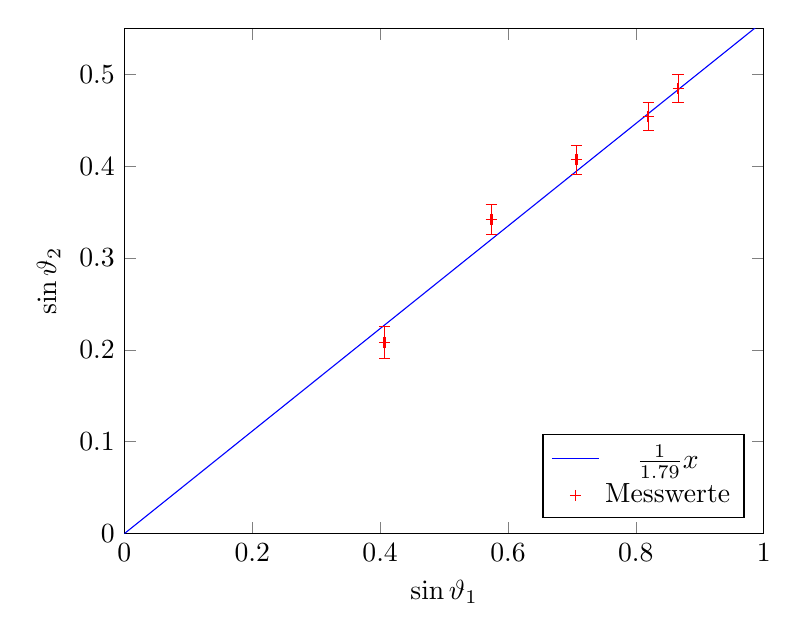
\begin{tikzpicture}
\begin{axis}[xmin = 0, ymin = 0, xmax = 1,
	legend pos = south east, width = .8\textwidth, height = 8cm,
	xlabel = $ \sin\vartheta_1 $,
	ylabel = $ \sin\vartheta_2 $]
	
	\addplot+[no marks, ] {1/1.7924933055*x};
	\addplot+[mark = +,only marks, error bars/.cd, x dir = both, x explicit, y dir=both, y explicit] table[x=x,y=y, x error = xerr, y error = yerr] {
x	y	xerr	yerr
0.4067366431	0.2079116908	0.0015944376	0.0170718962
0.5735764364	0.3420201433	0.00142969	0.0164007302
0.7071067812	0.4067366431	0.0012341341	0.0159443761
0.8191520443	0.4539904997	0.0010010797	0.0155509975
0.8660254038	0.4848096202	0.0008726646	0.0152649936
};
\legend{{$ \frac{1}{\num{1.79}}x $}, Messwerte}
\end{axis}
\end{tikzpicture}
\caption{$ \sin\vartheta_2 $ gegen $ \sin\vartheta_1 $ aufgetragen}
\label{fig:n}
\end{figure}
\subsection{title}
\newpage
\section{Diskussion} 
